\section{Experiments}

We evaluated SAMNet on the COG dataset and compared our results to the baseline model described in ~\cite{yang2018dataset}. To test the generalization ability of both models, we used the canonical (easy) and hard settings that alter the number of distractors and sequence length.  Since there was no baseline for these tests (train on canonical, test on hard), we ran our own experiments using the COG model provided by the authors.  SAMNet achieves the highest overall scores for all categories of experiments (Table 2), especially for the tests run on the hard dataset.  Among the 22 classification tasks, we highlighted the two most difficult tasks that affect the overall score.  More detailed results are provided in the Appendix.

We argue that the generalization capability of SAMNet is mainly due to the dynamic frame-by-frame processing of the input sequence.  The mechanisms introduced in SAMCell (e.g., Memory retrieval and update units) learn to operate independent of the total number of frames and allow to generalize to longer video lengths.  The visualization of the trained SAMNet model (see Appendix) indicates that the model learns the concept of time, helping it to control the flow of information from visual input to the memory.  Therefore, the memory is updated efficiently instead of storing all information across all frames.


%Our experiments were intended to study SAMNet's performances as well as generalization abilities in different settings. For this purpose, we use two different versions of the COG dataset, an easy one (canonical) and a hard version to explore a wide range of difficulties. The following parameters control the difficulty level: the number of frames in the input sequence, the maximum memory duration (how far is the last object to be remembered), and the number of distractors. These parameters are detailed in Table 1 for each setting. The table also shows the size of the training/validation/test split used for our experiments. The COG dataset is composed of 44 tasks that have equal number of samples.
%We chose to focus our effort only on the the 22 classification tasks.
%We compare our model to the original COG model  ~\cite{yang2018dataset} using their implementation (https://github.com/google/cog) and scores given by the authors. We also use the exact same training parameters detailed in the original paper.
%
%On the other side we trained SAMNet using IBM's Mi-Prometheus~\cite{kornuta2018accelerating}, a framework for research based on Pytorch. We trained all our models using NVIDIA’s GeForce GTX TITAN X GPUs. We trained  SAMNet using 8 reasoning steps SAMCells and a hidden state size of 128. The external memory has 128-bit slots. We trained our model until convergence but we also have set a training time limit of 80 hours.



\begin{table}[!t]
	\centering
	\caption{COG Dataset parameters for the canonical setting and the hard setting  }
	\resizebox{\textwidth}{!}{
	

	\begin{tabular}{ccccccc}
		\toprule
		
		Dataset    &  	number of frames  &  	maximum memory duration & number of distractors & size of training set & size of validation/test set    \\ 
          \midrule
		
		 Canonical setting & 4 & 3 & 1 & 10000320 & 500016 &   \\
		 \midrule
		 
		 Hard  setting & 8 & 7& 10 & 10000320 & 500016  \\
		 \bottomrule
	
	\end{tabular}
}

	
	\label{tab:parameters}
\end{table}


<<<<<<< HEAD
\subsection{Training and Implementation Details}
=======

\subsection{Training and testing Methodology}
>>>>>>> f2f4bdec46590da56efa04bb9c25eb405c8c3882

SAMNet is implmented on IBM's Mi-Prometheus~\cite{kornuta2018accelerating} framework based on Pytorch. 
We trained all our models using NVIDIA’s GeForce GTX TITAN X GPUs. SAMNet was trained using 8 reasoning steps and a hidden state size of 128. The external memory has 128-bit slots for all experiments. We trained our model until convergence but we also have set a training time limit of 80 hours.

We compared our model to the original COG model  ~\cite{yang2018dataset} using their implementation (https://github.com/google/cog) and scores provided by the authors through personal communications. We used the same training parameters detailed in the original paper and reproduced their results.  For the generalization experiments from canonical to hard, we used the verified model and obtained new results that were not reported in the reference paper.   In Table 2 COG section shows 4 columns divided into two parts: "paper" and "ours" which distinguish between the results reported in the paper vs. our own experiments.

Our experiments focused on the 22 classification tasks provided by the COG dataset.  First we evaluated SAMNet's performance on the canonical setting and compared it with the COG Model. As shown in Table 2 we could achieve a small improvement in accuracy, from 97.6\% for the COG model to 98\% for SAMNet. Next we focused on the hard setting of the dataset which increases the number of distractors from 1 to 10 and the number of frames from 4 to 8.

The first approach was to train a model on the hard training set, and test it on the hard test set. This is the same approach used by the COG paper ~\cite{yang2018dataset} to evaluate performance on the hard dataset. We achieve a test accuracy of 91.9 \% which represents a 12\% improvement from the COG model score (see Table 2).
%It shows that SAMNet's design choices make a difference when it come to harder tasks with longer sequences and more distractors objects.

The second approach was to see if the models can generalize from the easy to the hard setting. For this experiment, we trained a model on the canonical dataset, and directly tested on the hard dataset.  This experiment highlighted the most significant difference between SAMNet and the baseline COG model.

Finally we trained a model on the canonical data set, fine-tuned it on the hard data set using only 25k iterations, and tested on the hard dataset. Thanks to fine-tuning, we can observe a significant improvement from 91.6\%  to 96.5\% test accuracy which represents the state of the art accuracy for the hard setting (classification tasks).
After a short fine-tuning process, the transferred model could generalize well to harder tasks and even surpass the accuracy obtained in the first approach. We note that the third approach is also twice faster than the first one, and it is more effective in terms of accuracy.

A more granular analysis of accuracy per task shows a major improvement for the two hardest tasks, AndCompareShape and AndCompareColor. Those two tasks represent a higher level of difficulty due to the number of objects to be remembered in order to answer the question correctly.
As we can see in Table 2 we could achieve a 12\% improvement for the canonical data set and almost a 40\% improvement for the hard dataset.
The large improvement in these memory-intensive tasks indicate that the SAMNet's external memory plays a crucial role in our results.





\begin{table}[t]
	
	\caption{COG test set accuracies for  SAMNet \& COG models. For the COG section, the results marked as 'paper' comes from the original COG paper ~\cite{yang2018dataset}, whereas the results marked as 'ours' come from our own experiments using the following implementation: https://github.com/google/cog }
	
	\centering
	\resizebox{\textwidth}{!}{
	\begin{tabular}{ccccccccccc}
		\toprule
		Model & & SAMNet & && && COG&& \\
		\cmidrule{2-5} \cmidrule{7-11} 
		&&&&& & paper & ours & ours & paper&\\
		\cmidrule{7-9} \cmidrule{10-11}
		Trained on       & canonical & canonical & canonical & hard &           &  canonical  & canonical  & canonical & hard \\ 
		Fine tuned on  & - & - & hard  & - &           & -   & - & hard & - \\ 
		Tested on        & canonical & hard & hard & hard &            &canonical  & hard & hard & hard  \\ 
		\midrule
		
		Overall accuracy & 98.0 & 91.6 & 96.5  &  &           & 97.6  & 65.9 & & 80.1 \\ 
		
		\midrule 
		
		
		AndCompareColor	&	93.5		&	82.7	&	89.2	&&		&81.9	&57.1&  &	51.4
\\ 
		AndCompareShape	&	93.2 		&	83.7	&	89.7	&&	&	80.0	&53.1	& &50.7\\ 

		
		
		
		
		
		
		
		\bottomrule
	\end{tabular}
}
	\label{results}
\end{table}


\begin{figure}
	\centering
	\caption{Comparison of SAMNet and COG on their abilities to generalize from the canonical to the hard dataset. We show three different settings: 1) (baseline) trained on canonical, tested on canonical 2) trained on canonical, tested on hard, 3) trained on canonical, fine tuned on hard, tested on hard. }
	
	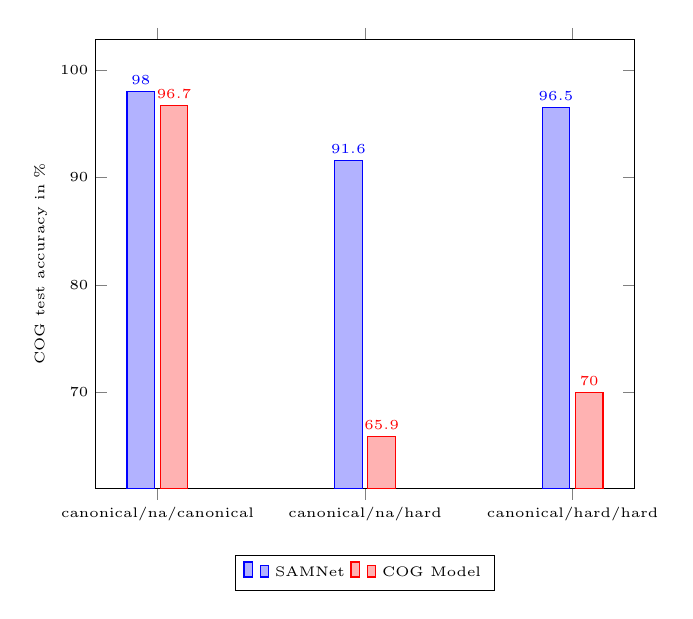
\begin{tikzpicture}
	
	
	
	\tiny
	
	\begin{axis}[
	ybar,
	enlargelimits=0.15,
	legend style={at={(0.5,-0.15)},
		anchor=north,legend columns=-1},
	ylabel={COG test accuracy in \% },
	symbolic x coords={canonical/na/canonical, canonical/na/hard, canonical/hard/hard},
	xtick=data,
	nodes near coords,
	nodes near coords align={vertical},
	]
	\addplot coordinates {(canonical/na/canonical,98) (canonical/na/hard,91.6) (canonical/hard/hard,96.5)};
	\addplot coordinates {(canonical/na/canonical,96.7) (canonical/na/hard,65.9) (canonical/hard/hard,70)};
	\legend{SAMNet ,COG Model}
	\end{axis}
	\end{tikzpicture}
\end{figure}


